\documentclass[../fem.tex]{subfile}

\begin{document}
\section{Localization}%
\label{sec:localization}

While it is occasionally possible to find the elements of the matrices in
equation \ref{eq:matrix_simp} on the global domain, this proves to be
exceedingly difficult in most if not all cases. To remediate this issue, we
implement a generalizable method that will work for any domain and and
functions that are being considered. Since we have the ability to select any
arbitrary basis functions as per our definition of the approximation to the
solution, then it is possible to select a basis such that it becomes
possible to split the domain into a finite number of subdomains.

We first discretize the domain $\Omega$ into $N$ mutually exclusive subdomains.
Each of these subdomains is called an \textit{element}. For the purposes of
this paper, each element will be defined to be a triangle subdomain of
$\Omega$. The set of all elements is called the triangular decomposition or the
mesh of the domain, the process for constructing the triangular decomposition
is discussed further in section \ref{sec:mesh_generation}. For the localization
process, the specifics of the triangular decomposition is not necessary, so we
will not go in depth on the structure of the triangular decomposition in this
section.

For each element of the mesh, we denote the element as $E^{(e)}$, where
$e=1,\ldots,N$. Then each vertex of the triangle is labeled as $E^{(e)}_i$
where $i=1,2,3$. The notation for the $x$ and $y$ values of each vertex we
denote as $X^{(e)}_i$ and $Y^{(e)}_i$ respectively, where $i=1,2,3$.

In 1D the process is trivial as all element have the same dimensions, but in
higher dimensional implementation, each element can have variable shapes and
sizes. This becomes more difficult because integrating over each element would
require entirely different process each time to account for the differences in
shape and size. To resolve this issue, we construct a master space, which is
possible to transition to from any element, and back to each element. Thus we
only need to determine a method to integrate over our master element.

\subsection{Master Space}%
\label{sub:master_space}

The master space is a domain that is constructed in order to simplify the
construction of the local approximations. For the situation with triangular
elements, we construct the master space such that the vertices of a triangle
lie on the points $(1,0,0)$, $(0,1,0)$, $(0,0,1)$. Then for each element in the
mesh, we construct a transformation between the master space and the element
space.

We define the master element to be $\widehat{E}$. An image of the master
element can be seen in figure \ref{fig:master_element}.

\begin{figure}[htpb]
  \begin{center}
    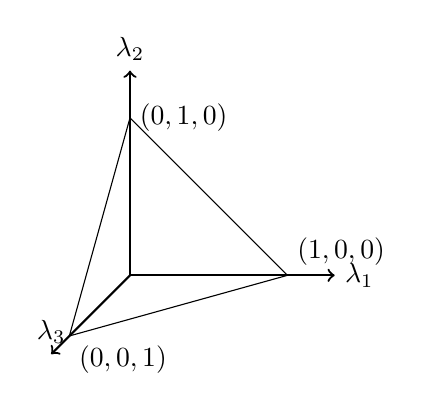
\begin{tikzpicture}[scale=2]
      \draw[thick,->] (0,0,0) -- (1.3,0,0) node[right]{$\lambda_1$};
      \draw[thick,->] (0,0,0) -- (0,1.3,0) node[above]{$\lambda_2$};
      \draw[thick,->] (0,0,0) -- (0,0,1.3) node[above]{$\lambda_3$};
      \draw (1,0,0) node[above right]{$(1,0,0)$}-- (0,1,0)
      node[right]{$(0,1,0)$} -- (0,0,1) node[below right]{$(0,0,1)$}-- cycle;
    \end{tikzpicture}
  \end{center}
  \caption{Master element $\widehat{E}$, in barycentric coordinate system, that
  is used instead of the variable local elements.}
  \label{fig:master_element}
\end{figure}

The master element utilizes what is called a Barycentric coordinate system. The
barycentric coordinates are demonstrated by each vertex being its own
dimension, so if the element were to be quadrangles, then the barycentric
coordinates would be in $\R^4$ instead of $\R^3$ as they are for triangles. The
conversion between the global coordinates and the Barycentric coordinates can
be done using the following equations
\begin{align*}
  \lambda_1&=\frac{(Y_2-Y_3)(x-X_3)+(X_3-X_2)(y-Y_3)}{(Y_2-Y_3)(X_1-X_3)+(X_3-X_2)(Y_1-Y_3)}\\
  \lambda_2&=\frac{(Y_3-Y_1)(x-X_3)+(X_1-X_3)(y-Y_3)}{(Y_2-Y_3)(X_1-X_3)+(X_3-X_2)(Y_1-Y_3)}\\
  \lambda_3&=1-\lambda_1-\lambda_2.
\end{align*}
Where $X_i$ and $Y_i$ represent the $x$ and $y$ coordinates of the $i$th vertex
of the element. $x$, $y$ are the coordinates of the point in the triangle that
is to be converted to the Barycentric coordinates. Converting from Barycentric
coordinates to the global coordinates uses the following equations
\begin{align*}
  x&=\lambda_1X_1+\lambda_2X_2+\lambda_3X_3\\
  Y&=\lambda_1Y_1+\lambda_2Y_2+\lambda_3Y_3
\end{align*}

\subsection{Local Basis}%
\label{sub:local_basis}

The first step is to construct a local basis function, that is only defined
for the current element under consideration. There should be a basis element
for every vertex in the element, so for triangular element, there will be three
local basis functions. The notation for the local basis functions is
$\ph^\e_1$, $\ph^\e_2$, and $\ph^\e_3$. To make computation simple, the
construct the basis function such that they are linear, with the requirement
that at the corresponding vertex, the local basis function is $1$ and at all
other vertices of the element the basis function will be $0$.

The conversion from global space to the bilinear coordinates does exactly this
task. Thus the definition of the local basis functions are
\begin{align}
  \begin{split}
    \ph^\e_1&=\frac{\left(Y^\e_2-Y^\e_3\right)\left(x-X^\e_3\right)+\left(X^\e_3-X^\e_2\right)\left(y-Y^\e_3\right)}{\left(Y^\e_2-Y^\e_3\right)\left(X^\e_1-X^\e_3\right)+\left(X^\e_3-X^\e_2\right)\left(Y^\e_1-Y^\e_3\right)}\\
    \ph^\e_2&=\frac{\left(Y^\e_3-Y^\e_1\right)\left(x-X^\e_3\right)+\left(X^\e_1-X^\e_3\right)\left(y-Y^\e_3\right)}{\left(Y^\e_2-Y^\e_3\right)\left(X^\e_1-X^\e_3\right)+\left(X^\e_3-X^\e_2\right)\left(Y^\e_1-Y^\e_3\right)}\\
    \ph^\e_3&=1-\ph^\e_1-\ph^\e_2.
  \end{split}
\end{align}

Thus for every element, there exist three local basis functions. A plot of
these local basis functions is shown in figure \ref{fig:local_basis} on an
arbitrary triangular element.

\begin{figure}[htpb]
  \begin{center}
    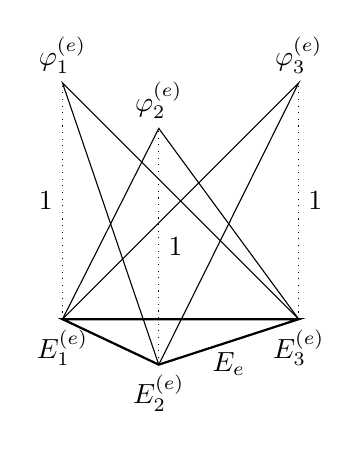
\begin{tikzpicture}[scale=3]
       \draw[thick] (0,0,0)node[below]{$E^{(e)}_1$} --
         (1,0,0)node[below]{$E^{(e)}_3$}
         --node[below]{$E_e$} (0.6, 0, 0.5)node[below]{$E^{(e)}_2$} -- cycle;
       \draw (0,1,0)node[above]{$\varphi_1^{(e)}$}  -- (1,0,0) -- (0.6, 0, 0.5)-- cycle;
       \draw (0,0,0) -- (1,1,0)node[above]{$\varphi_3^{(e)}$}  -- (0.6, 0, 0.5)-- cycle;
       \draw (0,0,0) -- (1,0,0) -- (0.6, 1, 0.5)node[above]{$\varphi_2^{(e)}$} -- cycle;
       \draw[dotted] (0,0,0) --node[left]{$1$} (0,1,0);
       \draw[dotted] (1,0,0) --node[right]{$1$} (1,1,0);
       \draw[dotted] (0.6,0,0.5) --node[right]{$1$} (0.6,1,0.5);
    \end{tikzpicture}
  \end{center}
  \caption{Plot of local basis function $\ph^\e_1$, $\ph^\e_2$, and $\ph^\e_3$,
  on some arbitrary element $E_e$.}
  \label{fig:local_basis}
\end{figure}


\subsection{Global Basis}%
\label{sub:global_basis}

The next step is to construct the global basis functions. Similarly to the
strategy for the construction of the local basis functions, each global basis
will be associated with a single vertex of the mesh. Thus for a mesh with $N$
elements, then there will be some number of global basis functions less than
$3N$. The method to define the global basis function is to define it to be $1$
at the associated vertex, and $0$ at all other vertices in the mesh.

In order to achieve this, the global basis function can be constructed as a
piecewise combination of $k$ different local basis functions, where $k$ is the
number of elements that share a given vertex. The exact formulation of the
global basis functions is dependent on the triangular mesh, and the current
vertex index. An example of what a global basis function could be like is
depicted in figure \ref{fig:global_basis}. One can intuitively think of the
global basis functions as $k$ sided pyramids this their peak directly above the
associated vertex.

\begin{figure}[htpb]
\begin{center}
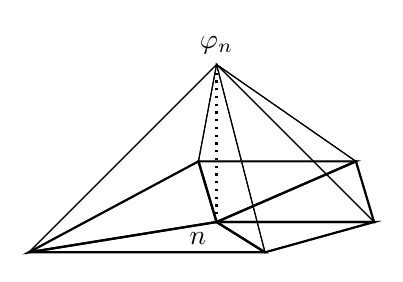
\begin{tikzpicture}[scale=1, transform shape]
          \draw (0,2,0) -- (1,0,-2) -- (2,0,0) -- cycle;
        \draw (0,2,0) -- (2,0,0) -- (1,0,1) -- cycle;
        \draw (0,2,0) -- (1,0,1) -- (-2,0,1) -- cycle;
        \draw (0,2,0) -- (-2,0,1) -- (-1,0,-2) -- cycle;
        \draw (0,2,0) -- (-1,0,-2) -- (1,0,-2) -- cycle;

        \draw[thick] (0,0,0) -- (1,0,-2) -- (2,0,0) -- cycle;
        \draw[thick] (0,0,0) -- (2,0,0) -- (1,0,1) -- cycle;
        \draw[thick] (0,0,0) -- (1,0,1) -- (-2,0,1) -- cycle;
        \draw[thick] (0,0,0) -- (-2,0,1) -- (-1,0,-2) -- cycle;
        \draw[thick] (0,0,0) -- (-1,0,-2) -- (1,0,-2) -- cycle;

        \draw[dotted, thick] (0,0,0)node[below left]{$n$} -- (0,2,0) node[above]{$\varphi_n$};
\end{tikzpicture}
\end{center}
\caption{Global basis function $\ph_n$, demonstrating a potential shape of the
global basis functions on a limited portion of a triangular mesh.}
\label{fig:global_basis}
\end{figure}


\subsection{Local System}%
\label{sub:local_system}

Using the definition of local basis functions that were constructed in section
\ref{sub:local_basis}, the construction of an element-specific system of
equations is performed. The system of equations is identical to the global
system but is simply specified to a single element. Thus the local system of
equations in matrix form is
\begin{align*}
  G^\e\partial_t U^\e=\left(\wb{A}^\e+\wb{B}^\e+\wb{C}^\e\right)U^\e+F^\e.
\end{align*}

In this system of equations, the elements of each matrix are only determined by
the local basis function on the element $e$. The size of the matrix is
equivalent to the number of vertices in the element, thus for the triangular
element case, the matrices have a size of three. The element of these matrices
can be found through the following equations
\begin{align}\label{eq:local_sys}
  \begin{aligned}
    G^\e_{ij} &=\int_{E_e}\ph^\e_i\ph^\e_jdA\quad &i,j&=1,2,3\\
    \wb{A}^\e_{ij}&=-\sum_{\alpha,\beta=1}^2\int_{E_e}\pder{\ph^\e_j}{x^\beta}\pder{}{x^\alpha}\left(A_{\alpha\beta}\ph^\e_i\right)dA\quad
                  &i,j&=1,2,3\\
    \wb{B}^\e_{ij}&=\sum_{\gamma=1}^2\int_{E_e}B^\gamma\ph^\e_i\pder{\ph^\e_j}{x^\gamma}dA\quad
                  &i,j&=1,2,3\\
    \wb{C}^\e_{ij}&=\int_{E_e}C\ph^\e_i\ph^\e_jdA\quad &i,j&=1,2,3\\
    F^\e_i&=\int_{E_e}\ph^\e_ifdA\quad & i&=1,2,3.
  \end{aligned}
\end{align}

Using only the local matrix elements, it is possible to construct the global
system, utilizing some specific algorithms that are discussed in section
\ref{sec:assembly_of_the_global_system}.

\end{document}
